\chapter{Introducción}


\section{El marketing digital en la web}


\subsection{¿Qué és?}

El marketing digital son técnicas y estrategias de comercialización usando medios digitales, tales como dispositivos móviles, televisiores digitales y ordenadores.

\vspace{5 mm}

\textbf{¿Cuáles son las principales diferencias respecto al marketing tradicional?} 

\vspace{5 mm}

\begin{itemize}

\item \textbf{Personalización}: El marketing digital pretende obtener información del usuario más personalizada. Por ello aplica técnicas que permiten que se le sugieran a los internautas información de aquello que está interesado, basado en búsquedas previas o en sus preferencias definidas.

\item \textbf{Masivo}: Se puede obtener un gran número de usuarios que formen parte de tu público objetivo invirtiendo muchos menos dinero que en el marketing tradicional.


\end{itemize}

\subsection{Evolución}

La concepto de marketing digital en la web durante sus inicios hasta la actualidad ha ido ido variando. En los años noventa con la aparición de los primeros banners, aparecen las primeras técnicas de marketing en páginas web aunque este primer concepto que se tiene es mucho más básico y se basaba principalmente en hacer publicidad hacia los usuarios para captar posibles clientes.

\vspace{5 mm}


Con la llegada de las redes sociales y la aparición de los smartphones el concepto de marketing cambia, no se basa únicamente en promocionar un producto. Se pretende crear una estrategia de venta basada en la perspectiva del cliente. Reconociendo e investigando en las áreas que ayuden a los clientes a pensar que sus opiniones importan, genera una fidelidad hacia la marca. Aquí es donde las redes sociales juegan un gran papel, ya que permiten compartir todo tipo de contenido(videos,enlaces,textos) que se asocian a nuestras opiniones y gustos personales. Todo este contenido permite a las empresas conocer más detalladamente a un potencial cliente y así crear estrategías de marketing para fidelizar con él.


\subsection{Técnicas}

Una web es uno de lo mejores sitios para incrementar el prestigio y visibilidad de una marca y alcanzar un mayor rango de clientes con efectividad. Para ello, entran en juego diversas técnicas de marketing digital que nos permiten obtener una mayor visibilidad de marca:

\vspace{5 mm}

\textbf{Posicionamiento SEO}

\vspace{5 mm}

\begin{figure}
\begin{center}
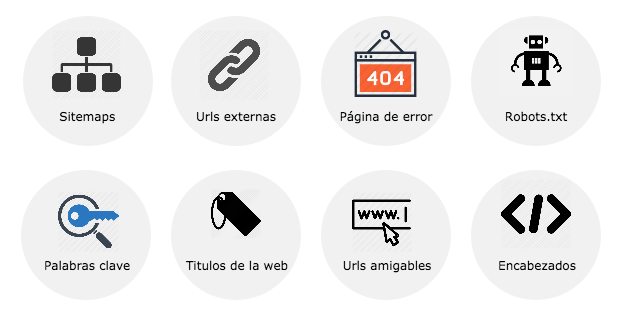
\includegraphics[width=1.0\textwidth]{imagenes/SEO.png}
\caption{Técnicas de SEO}
\label{SEO}
\end{center}
\end{figure}

El posicionamiento en buscadores mejor conocido como posicionamiento SEO es un conjunto de técnicas que implican una mejora de la página web con el fin de mejorar su posición en los resultados de los buscadores para unos términos de búsqueda específicos. Cuanto mejor esta optimizada la página web obtiene una mejor posición en los buscadores y por tanto una mayor visibilidad. En la figura \ref{SEO} se observan las principales técnicas de posicionamiento SEO, que se describen a continuación:

\begin{itemize}

\item \textbf{keywords}: palabras clave, son un conjunto de datos asociados a la página que tienen relación con una posible búsqueda por parte de los usuarios en un buscador. Se asocian como metadatos a una página de la web y son unos de los elementos más básicos para el posicionamiento SEO.

\item \textbf{Urls amigables}: usar palabras cortas y amigables como Urls en el sitio web de vez de urls complejas, permite al buscador disponer de palabras clave para interpretar su contenido. Además es mucho más fácil de interpretar por las personas.

\item \textbf{Etiquetas de Título}: cada página del sitio web, tiene unos metadatos asociados. Una de las etiquetas es el title(título), que indica el nombre de la página web. Es importante que cada página de la web tenga un título diferente y que el texto tenga una información relacionada con la página para facilitar la indexación por parte de los buscadores.

\item \textbf{Mapa de contenido del sitio}: conocido como sitemaps(en inglés), es una lista de las páginas del sitio con información adicional tal como la importancia de la página o la frecuencia con la que cambia de contenidos. Generalmente los sitemaps se generan como fichero XML.

\item \textbf{Página de error personalizada}: una página de error amigable y personalizada mejora la experiencia para el usuario y evita problemas de indexación por parte de los buscadores.

\item \textbf{Insertar links externos}: tener enlaces de otras páginas respetables por los buscadores favorece también a tu sitio al buen posicionamiento.

\item \textbf{Fichero robots}: fichero txt que sirve de guía para los buscadores sobre que información de el sitio web rastrear para posicionarla. Mediante este fichero se delimitan que páginas no queremos que aparezcan posicionadas(página de admin o de política de privacidad por ejemplo) y facilitando la lectura de los crawlers(rastreadores) en el sitio.

\item \textbf{Encabezados de la página}: Utilizar las etiquetas de encabezado(h1,h2,h3) correctamente estableciendo una jerarquía en tu web y utilizados como palabras clave.  


\end{itemize}

\vspace{5 mm}

\textbf{La analítica web}

\vspace{5 mm}

La analítica web nos permite estudiar la repercusión de las campañas de marketing online. Con esta técnica se pretende entender el tráfico del sitio web y así implementar nuevas mejoras en la web.

\vspace{5 mm}

En los inicios de la analítica, el objetivo principal se basaba en medir el número de visitas de un portal web, cuantas más visitas una mayor probabilidad de generar publicidad. En la actualidad se siguen analizando el numero de visitas de un sitio, pero la analítica web sigue evolucionando y se empiezan a medir otros indicadores como la profundidad de las visitas. Las métricas mas importantes utilizadas se dividen en dos tipos, básicas y avanzadas.


\textbf{Métricas básicas}: Nos permiten ver el tráfico en la web: 

\begin{itemize}

\item \textbf{Visitas}: Número de visitas de la página.

\item \textbf{Tasa de rebote}: Mide el número de personas que llegan a una determinada página del sitio.

\item \textbf{Tasa de salida}: Conocer las páginas de la web en las que los visitantes abandonan la web.

\item \textbf{Fuentes de tráfico}: Analiza las fuentes de donde provienen las visitas de los usuarios. 

\end{itemize}

\vspace{5 mm}

 \textbf{Métricas avanzadas(KPI)}: indicadores clave del rendimiento del sitio web. Estás metricas se basan en la comparación de los objetivos marcados por la empresa a lo conseguido. En función del tipo del sitio web los KPIs serán diferentes:

\begin{itemize}

\item \textbf{Sitio web de contenido}: para un sitio web de contenidos los objetivos principales son captar tráfico y fidelizar con el usuario de forma que vuelva otra vez al sitio web. Para este sitio se emplearían KPIs tales como:

- La profundidad de las visitas. Tasa que mide la cantidad de páginas de la web que ve un usuario en una visita.

- Tasa de conversion. Porcentaje que se obtiene del número de conversiones entre el número de visitas. Las conversiones. La definición de conversión dependerá del tipo de web. Para un sitio con contenidos las conversiones equivalen al número de registros en la aplicación.

\item \textbf{Sitio web de ventas}: El objetivo principal de una tienda online es conseguir el mayor número de ventas. Para ello  se utilizarían los siguientes KPIs:

- Ingresos por visita. Porcentaje que expresa el número de ingreso de la tienda en función del número de visitas a la web.

- Cantidad media por pedido. Esta tasa mide la cantidad total de ingresos obtenidos por la empresa entre el número de ventas realizadas.

\end{itemize}

\begin{figure}
\begin{center}
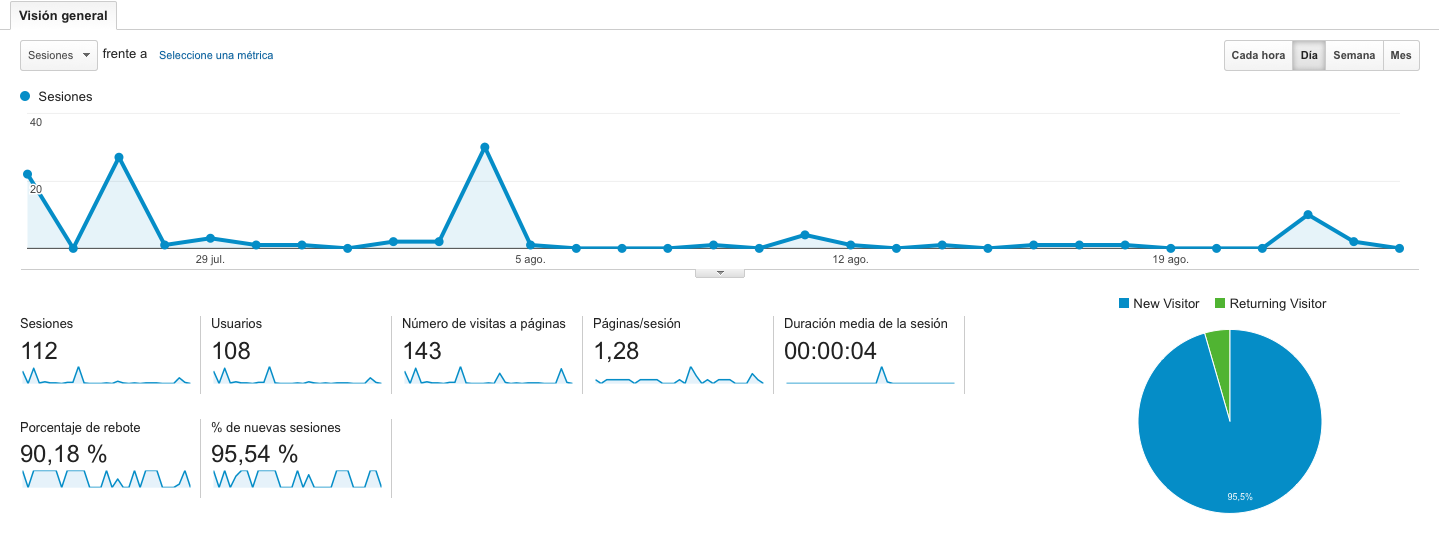
\includegraphics[width=1.0\textwidth]{imagenes/analytics.png}
\caption{Panel de analytics}
\label{analytics}
\end{center}
\end{figure}

Para monitorizar toda el tráfico de datos obtenido de las métricas aplicadas se usan herramientas de analítica web. Una excelente herramienta gratis es Google Analytics, que proporciona un dashboard muy completo para monitorizar la información de tu sitio web.

\textbf{La redes sociales} 

\vspace{5 mm}

Con la aparición de las redes sociales y su gran apogeo entre los usuarios de internet, las empresas ven una herramienta muy potente para promover sus marcas. Las principales técnicas de social media marketing, adaptadas a las necesidades de cada empresa  puede reportar muchos beneficios:

\begin{itemize}

\item \textbf{Difusión}: se consigue una difusión de la información rápida y económica.

\item \textbf{Recopilación de datos}: Se obtiene una gran cantidad de información(BIG DATA) sobre el público objetivo de la marca utilizando una táctica para las redes sociales.

\item \textbf{Mayor número de visitas}: Mediante la difusión de contenido en redes sociales y con una buena táctica bien orientada se consigue una mayor visibilidad de tu sitio web.

\end{itemize}

Como se dice previamente, del uso de tácticas de social media, se obtiene una recopilación de datos relevante para ser utilizados por una empresa con el fin de afianzar la fidelidad con sus clientes o conseguir nuevos. Con los datos obtenidos de las redes sociales las empresas pueden analizar la información y utilizarla sabiamente para dar una mayor visibilidad a su marca. Un ejemplo de uso de los datos de redes sociales podría ser la obtención de un segmento del mercado, donde los potenciales clientes poseen unas características y necesidades similares(un nicho de mercado) sobre el que la empresa pueda generar un nuevo modelo de negocio.


\subsection{Targeting de las redes sociales}

Aunque todas las redes sociales se emplean generalmente para dar una mayor visibilidad,para conseguir un resultado satisfactorio, se debe elegir previamente la red social adecuada que usan los potenciales clientes del producto. 

\vspace{5 mm}

Actualmente existen muchas redes sociales enfocadas a diferentes ámbitos: Linkedin(ámbito profesional),Pinterest(ámbito artistico), Facebook(ámbito social). Cualquiera de las redes sociales actuales se puede emplear como target de un producto o marca, aunque generalmente se usan las que tienen un mayor número de usuarios ya que existe una mayor facilidad de encontrar un nicho de mercado.Tres redes sociales más usadas en el mundo son: la web de microblogging Twitter, la web social de amistades Facebook y la aplicación de fotografía Instagram.

\vspace{5 mm}

\section{Big Data}

\subsection{¿Qué és?}

Big Data se concibe como la gestión y análisis de grandes cantidades de información.Big data nos proporciona soluciones que utilizando métodos convencionales llevaría un tiempo mucho más elevado.

\subsection{Las 3Vs}

Todo el volumen de información puede provenir de diferentes tipos de fuentes. En Big data se definen 3 tipos de propiedades de los datos(ver figura \ref{3vs}):

\begin{itemize}

\item \textbf{Volumen de datos}: hace referencia a el tamaño de los datos.

\item \textbf{Variedad de datos}: se refiere a los distintos tipos de datos

\item \textbf{Velocidad de datos}: la velocidad con la que se procesan los datos.

\end{itemize}

\begin{figure}
\begin{center}
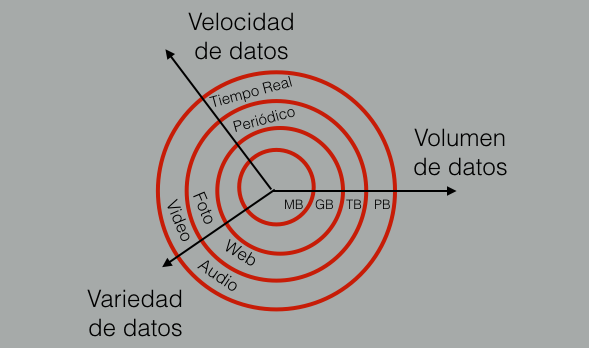
\includegraphics[width=1.0\textwidth]{imagenes/3V.png}
\caption{Las 3Vs de Big Data}
\label{3vs}
\end{center}
\end{figure}

\section{Enfoque Principal}

Ya se han detallados los conceptos clave sobre los que se basa el proyecto. La idea general del proyecto es la de una aplicación web social de ámbito culinario. Para elaborarlo se utilizarán herramientas como \textbf{Técnicas de Marketing Digital} y \textbf{Big Data}. Se pretende cónocer como dar una mayor visibilidad de la aplicación y captar un mayor número de usuarios(técnicas de marketing) y asi obtener un nicho de mercado sobre el que basar el modelo de negocio del proyecto(Big Data).

